% Updated from executed/31_grpo.ipynb and pages/31-grpo*.md.

\chapter[GRPO 정렬]{GRPO: 검증 가능한 보상으로 정렬}
\label{ch:31}
\markboth{GRPO 정렬}{GRPO 정렬}

\chaptermeta{31_grpo/31_grpo.ipynb}{https://colab.research.google.com/github/yoon-gu/neuqes-101/blob/master/31_grpo/31_grpo.ipynb}{preference 쌍 대신 verifier가 자동 채점하는 reward로 policy를 정렬하는 GRPO 학습 단계}

\index{1GRPO@GRPO}
\index{1Group Relative Policy Optimization@Group Relative Policy Optimization}
\index{1verifiable reward@verifiable reward}
\index{1verifier@verifier}
\index{1group relative advantage@group relative advantage}
\index{1reward std@reward std}
\index{1rollout group@rollout group}
\index{1reward 0@reward=0}
\index{1std 0@std=0}
\index{1advantage 0@advantage=0}
\index{1group mean@group mean}
\index{1baseline@baseline}
\index{1critic free RL@critic-free RL}
\index{1GRPOTrainer@GRPOTrainer}
\index{1GRPOConfig@GRPOConfig}
\index{1num generations@num\_generations}
\index{1format reward@format reward}
\index{1correctness reward@correctness reward}
\index{1verifier pass rate@verifier pass rate}
\index{1arithmetic reward@arithmetic reward}
\index{1base capability@base capability}
\index{1reward hacking@reward hacking}
\index{1RL before SFT@RL before SFT}
\index{1DeepSeek R1@DeepSeek-R1}
\index{1DeepSeek R1 style@DeepSeek-R1 style}
\index{1Qwen appendix@Qwen appendix}
\index{1Qwen2 5 0 5B Instruct@Qwen2.5-0.5B-Instruct}
\index{1HPO@HPO}
\index{1hyperparameter@hyperparameter}
\index{1temperature@temperature}
\index{1learning rate@learning\_rate}
\index{1beta 0 0@beta=0.0}
\index{1max steps@max\_steps}
\index{1SFT warm start@SFT warm-start}
\index{1difficulty filter@difficulty filter}
\index{1dr grpo@dr\_grpo}
\index{1fp16 AMP@fp16 AMP}
\index{1fp32 load@fp32 load}
\index{1dtype@dtype}
\index{1Diffusion LM@Diffusion LM}
\index{1Phase 5@Phase 5}
\index{0검증 가능한 보상@검증 가능한 보상}
\index{0검증기@검증기}
\index{0그룹 상대 어드밴티지@그룹 상대 어드밴티지}
\index{0롤아웃 그룹@롤아웃 그룹}
\index{0보상 0@보상 0}
\index{0보상 표준편차@보상 표준편차}
\index{0기준선@기준선}
\index{0그룹 평균@그룹 평균}
\index{0자동 채점@자동 채점}
\index{0산술 보상@산술 보상}
\index{0정답 보상@정답 보상}
\index{0형식 보상@형식 보상}
\index{0기반 능력@기반 능력}
\index{0능력 증폭@능력 증폭}
\index{0보상 해킹@보상 해킹}
\index{0난이도 필터@난이도 필터}
\index{0워밍스타트@워밍스타트}
\index{0하이퍼파라미터@하이퍼파라미터}
\index{0형식 준수@형식 준수}
\index{0Diffusion 언어모델@Diffusion 언어모델}

\section{누적 추적표}

\begin{booktable}{31장 누적 추적표}{tab:ch31-trace}
\begin{adjustbox}{max width=\textwidth}
\begin{tabular}{@{}llllll@{}}
\toprule
장 & 단계 & 모델 & 데이터 & 신호 & Trainer \\
\midrule
\ref{ch:28}장 & SFT & KoGPT2 & instruction-response & 답변 토큰 CE & \inlinecode{SFTTrainer} \\
\ref{ch:30}장 & DPO & policy + reference & chosen/rejected & preference margin & \inlinecode{DPOTrainer} \\
\textbf{31장} & \textbf{GRPO} & \textbf{SFT warm-start policy} & \textbf{prompt + 정답} & \textbf{verifier reward} & \textbf{\inlinecode{GRPOTrainer}} \\
\bottomrule
\end{tabular}
\end{adjustbox}
\end{booktable}

\section{변경점: preference 쌍에서 verifier 보상으로}

DPO는 같은 prompt에 대한 \inlinecode{chosen}/\inlinecode{rejected} 쌍을 비교했습니다. GRPO는 모델이 한 prompt에 대해 여러 답을 직접 생성하고, verifier가 각 답을 자동 채점합니다. 같은 prompt 안의 reward 평균을 baseline으로 쓰기 때문에 별도 critic이 필요 없습니다.

\begin{equation}
A_i =
\frac{r_i - \operatorname{mean}(r_1,\ldots,r_G)}
     {\operatorname{std}(r_1,\ldots,r_G)+\varepsilon}.
\label{eq:ch31-advantage}
\end{equation}

\eqref{eq:ch31-advantage}에서 모든 답의 reward가 같으면 표준편차가 0에 가깝고 advantage도 0이 됩니다. 이 장의 핵심은 이 조건을 실제로 다루는 것입니다. 산술 문제는 정답이 자동 검증되므로 GRPO를 설명하기 좋지만, 작은 모델은 prompt별 정답률이 0 또는 1로 양극화되기 쉽습니다. 따라서 SFT warm-start와 난이도 필터가 필요합니다.

\section{PPO, DPO, GRPO 비교}

\begin{booktable}{31장 alignment 방법 비교}{tab:ch31-methods}
\begin{adjustbox}{max width=\textwidth}
\begin{tabular}{@{}llll@{}}
\toprule
방법 & 학습 신호 & 필요한 모델 & T4 관점 \\
\midrule
PPO & reward model 점수 & policy, reference, reward, critic & 무겁습니다 \\
DPO & preference pair & policy, frozen reference & T4에서 가능 \\
GRPO & verifier reward + group baseline & policy, 선택적 reference & critic 없이 가능 \\
\bottomrule
\end{tabular}
\end{adjustbox}
\end{booktable}

GRPO는 DPO와 경쟁한다기보다 다른 종류의 alignment입니다. 주관적 품질, 안전성, 말투는 DPO나 judge 기반 선호 학습이 적합하고, 수학·코드처럼 정답 검증이 가능한 task는 GRPO가 적합합니다.

\section{실습: 산술 데이터와 verifier}

\begin{lstlisting}
def make_prompt(a, b):
    return (
        "### Instruction:\n"
        f"{a} + {b} = ?\n\n"
        "### Response:\n"
    )

def extract_last_int(text):
    found = re.findall(r"-?\d+", text)
    return found[-1] if found else None

def reward_correct(completions, answer, **kwargs):
    rewards = []
    for text, gold in zip(completions, answer):
        pred = extract_last_int(text)
        rewards.append(1.0 if pred == str(gold) else 0.0)
    return rewards
\end{lstlisting}

\noindent\emph{위 코드 읽기.}
\inlinecode{make\_prompt}는 KoGPT2 SFT에서 쓴 instruction 형식을 맞춥니다. \inlinecode{reward\_correct}는 생성 답변에서 마지막 정수를 뽑아 정답과 같으면 1, 아니면 0을 줍니다. 보상은 이진이지만 사람이 채점하지 않습니다.

\begin{bookoutputbox}
train: 256 samples,  eval: 64 samples

### 명령어:
7 + 7 = ?

### 응답:
answer: 14
\end{bookoutputbox}

\section{SFT warm-start}

이전 원고의 cold-start 실험은 중요한 실패 조건을 보여 줬지만, 최신 검증본은 그 조건을 해결하는 방향으로 갱신됐습니다. 먼저 짧은 SFT로 산술 응답 형식을 가르칩니다. 이 단계의 목적은 reasoning을 완성하는 것이 아니라, GRPO가 증폭할 수 있는 초기 성공률을 만드는 것입니다.

\begin{bookoutputbox}
SFT warm-start done (1.2min) - policy now knows arithmetic format
\end{bookoutputbox}

실행본 기준으로 SFT warm-start 후 greedy 평가 정확도는 0.875입니다. cold-start의 0\% 상태와 달리 이제 group 안에 정답과 오답이 섞일 가능성이 생깁니다.

\section{group advantage 손계산}

\begin{lstlisting}
def group_advantage(rewards, eps=1e-8):
    r = np.asarray(rewards, dtype=np.float32)
    return (r - r.mean()) / (r.std() + eps)

print(group_advantage([1, 1, 1, 1]))
print(group_advantage([0, 1, 0, 1]))
\end{lstlisting}

\begin{bookoutputbox}
rewards=[1,1,1,1] -> advantage=[0. 0. 0. 0.] (all same -> no learning signal)
rewards=[0,1,0,1] -> advantage=[-1.  1. -1.  1.] (mixed -> usable signal)
\end{bookoutputbox}

\textbf{출력 해석.}
GRPO가 작동하려면 group reward가 섞여야 합니다. 모든 답이 정답이어도, 모든 답이 오답이어도 상대 advantage는 0입니다. 이 때문에 산술 prompt를 전부 쓰지 않고 난이도 필터를 둡니다.

\section{난이도 필터}

한 자리 산술은 prompt에 따라 너무 쉽거나 너무 어렵습니다. SFT 모델이 항상 맞히는 prompt는 GRPO 신호가 없고, 항상 틀리는 prompt도 신호가 없습니다. 실행본은 SFT 후 정답률이 25\%에서 87.5\% 사이인 prompt만 GRPO 학습셋으로 골랐습니다.

\begin{bookoutputbox}
BEFORE GRPO - arithmetic accuracy (greedy verifier pass rate): 0.875
난이도 필터: pool 500 -> 중간난이도 256개
(그룹에 정답·오답 섞임 -> advantage std>0)
\end{bookoutputbox}

\textbf{출력 해석.}
GRPO의 병목은 reward 함수가 아니라 reward 분산입니다. 난이도 필터는 verifier reward의 표준편차가 0으로 사라지는 구간을 줄이는 장치입니다.

\section{\inlinecode{GRPOConfig}: 붕괴를 피하는 설정}

최신 실행본은 \inlinecode{trl} 1.6.0 기준으로 안정적인 GRPO 설정을 사용합니다. 핵심은 작은 learning rate, \inlinecode{dr\_grpo} loss, reward scaling 비활성화, 약한 KL 제약입니다.

\begin{lstlisting}
grpo_config = GRPOConfig(
    output_dir="./out_kogpt2_grpo",
    learning_rate=5e-6,
    loss_type="dr_grpo",
    scale_rewards=False,
    beta=0.04,
    max_grad_norm=0.2,
    num_generations=8,
    max_completion_length=24,
    fp16=True,
    report_to="none",
)
\end{lstlisting}

\noindent\emph{위 코드 읽기.}
\inlinecode{learning\_rate=5e-6}과 \inlinecode{max\_grad\_norm=0.2}는 작은 모델에서 정책이 급격히 무너지는 것을 막습니다. \inlinecode{scale\_rewards=False}는 이진 verifier reward를 그대로 쓰겠다는 뜻입니다. \inlinecode{beta=0.04}는 reference와 너무 멀어지지 않도록 약한 KL 제약을 둡니다.

\begin{bookoutputbox}
=== GRPO summary ===
elapsed     : 0.49 min
global_step : 32
train_loss  : 5171634.2480
final peak  : 2886 MiB
\end{bookoutputbox}

GRPO의 \inlinecode{train\_loss}는 일반적인 cross entropy loss처럼 읽으면 안 됩니다. reward, reward std, verifier pass rate를 함께 봐야 합니다.

\section{GRPO 전후 결과}

\begin{bookoutputbox}
AFTER  GRPO - arithmetic accuracy (verifier pass rate): 0.891
BEFORE GRPO - arithmetic accuracy                     : 0.875
delta                                                 : +0.016
\end{bookoutputbox}

\begin{bookfigurelabel}[H]{KoGPT2 GRPO 전후 산술 verifier 통과율}{fig:ch31-grpo-kogpt2-accuracy}
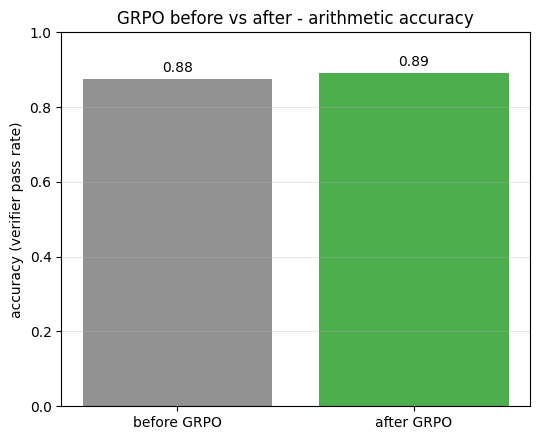
\includegraphics[width=0.72\linewidth]{assets/figures/ch31_grpo_kogpt2_accuracy.png}
\end{bookfigurelabel}

\textbf{그림 읽기.}
그림~\ref{fig:ch31-grpo-kogpt2-accuracy}는 SFT warm-start 이후 GRPO가 산술 verifier pass rate를 0.875에서 0.891로 올린 결과를 보여줍니다. 변화폭은 작지만, cold-start에서 reward가 모두 0이던 상황과 달리 실제 개선이 관찰됩니다.

\begin{bookoutputbox}
peak VRAM (max over training): 3670 MiB
(policy + weak KL anchor, beta=0.04, num_generations=8, fp16)
\end{bookoutputbox}

\begin{bookfigurelabel}[H]{KoGPT2 GRPO 학습 중 reward와 VRAM 흐름}{fig:ch31-grpo-kogpt2-curves}
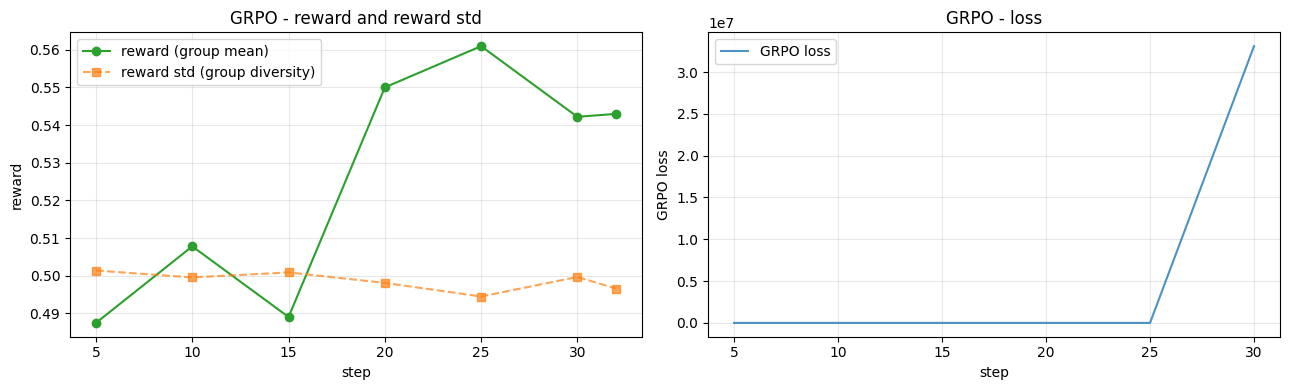
\includegraphics[width=0.88\linewidth]{assets/figures/ch31_grpo_training_curves.png}
\end{bookfigurelabel}

\textbf{그림 읽기.}
그림~\ref{fig:ch31-grpo-kogpt2-curves}는 GRPO가 rollout을 포함해도 T4에서 policy 중심으로 실행 가능하다는 점을 보여줍니다. peak VRAM은 3670 MiB입니다.

\section{핵심 해석}

본 장의 결론은 “GRPO가 산술을 새로 발명했다”가 아닙니다. SFT warm-start로 모델이 이미 산술 형식과 일부 정답을 내게 만들고, 난이도 필터로 group reward의 표준편차를 살린 뒤, GRPO가 그 신호를 조금 증폭했습니다. 즉 GRPO는 능력 생성보다 능력 증폭에 가깝습니다.

\begin{faqBox}{Q1. GRPO는 DPO와 언제 다르게 쓰나요?}
DPO는 사람이 선호하는 답변 쌍이 있을 때 적합합니다. GRPO는 수학, 코드 테스트, 형식 검증처럼 정답을 자동 판정할 수 있을 때 적합합니다.
\end{faqBox}

\begin{faqBox}{Q2. 왜 SFT warm-start가 필요한가요?}
모델이 한 번도 맞히지 못하면 모든 reward가 0이 됩니다. 그러면 \eqref{eq:ch31-advantage}의 advantage가 0이 되어 업데이트 방향이 사라집니다. SFT는 GRPO가 증폭할 최소한의 성공률을 만듭니다.
\end{faqBox}

\begin{faqBox}{Q3. 난이도 필터는 데이터 누수인가요?}
평가셋을 골라 성능을 부풀리는 용도가 아니라, 학습 prompt 중 group reward가 섞일 가능성이 있는 항목을 고르는 장치입니다. 최종 평가는 별도 eval 셋에서 확인합니다.
\end{faqBox}

\begin{faqBox}{Q4. \inlinecode{train\_loss}가 너무 큰데 실패 아닌가요?}
GRPO loss는 CE처럼 직관적으로 해석하기 어렵습니다. 이 장에서는 verifier pass rate, reward std, VRAM 흐름을 함께 봅니다.
\end{faqBox}

\begin{faqBox}{Q5. DeepSeek-R1과의 연결은 무엇인가요?}
공통점은 verifiable reward입니다. 정답을 자동 검증할 수 있는 문제에서 여러 답을 생성하고, 그중 더 좋은 답을 상대적으로 강화합니다. 차이는 규모와 base 능력입니다.
\end{faqBox}

\begin{previewBox}{미리보기: 다음 Phase}
\ref{ch:32}장부터는 autoregressive 생성의 전제를 잠시 내려놓고 diffusion LM으로 넘어갑니다. 한 토큰씩 쓰는 대신 전체 시퀀스를 \inlinecode{[MASK]}에서 병렬로 복원하는 생성 방식을 실험합니다.
\end{previewBox}
